% Chapter Template

\chapter{Background} % Main chapter title

\label{Chapter3} % Change X to a consecutive number; for referencing this chapter elsewhere, use \ref{ChapterX}

\lhead{Chapter 3. \emph{Background}} % Change X to a consecutive number; this is for the header on each page - perhaps a shortened title

%----------------------------------------------------------------------------------------
%	SECTION 1
%----------------------------------------------------------------------------------------
Before discussing implementation details and research questions, we provide a brief description of the SWAN program.
The first subsection will focus only on key features of SWAN, relevant to our work.
The second chapter will briefly describe few Beacon Frame Standards relevant for our research.

\section{SWAN}
The core functionality of the SWAN is to act as a middleware between the phone applications and the actual hardware or software sensors.

The application's interface with SWAN is always the same, the only component that vary is the SWAN Song expression passed to SWAN.

Swan Song Expression(\hyperref[fig:SwanExpression]{Figure 3.1}) encapsulate all the information required by SWAN.
Beside passing data to application, SWAN also takes care of evaluation and storage. Relevant parameters are also embedded into the 
SWAN Song expression.

\begin{figure}[htbp]
  \centering
    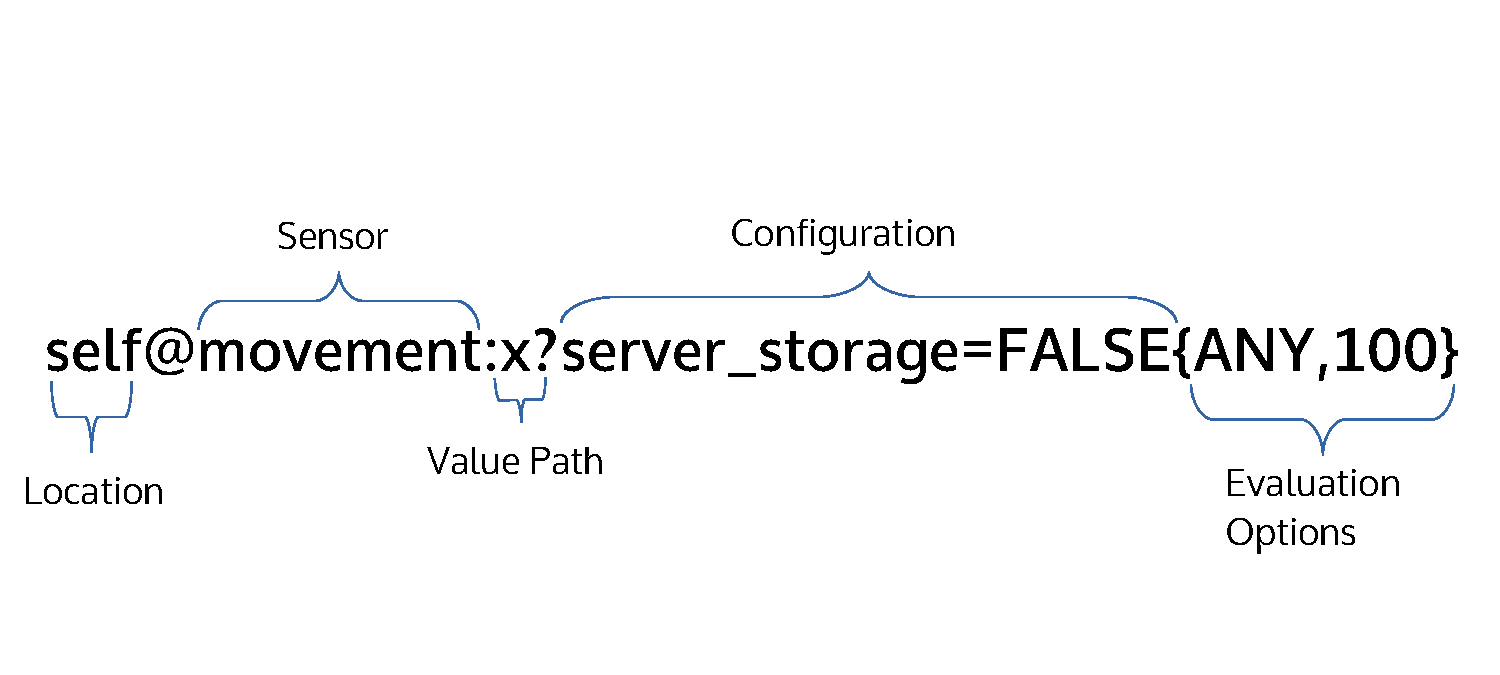
\includegraphics[scale=0.6]{Figures/swan_expr.pdf}
    \rule{35em}{0.5pt}
  \caption[Swan Expression]{Detailed swan expression).}
  \label{fig:SwanExpression}
\end{figure}

As part of our research we will also operate changes on the SWAN Song Expression and the meaning of different parameters.

\section{Beacon Frame Standards}
With Bluetooth Low Energy devices market in its incipient stage, the Beacon  emitters suffer from high fragmentation.
To help improve the situation, Apple and Google stepped up to offer frame specifications and further enforce the standard.

Apple's format, called iBeacon is simple and only focused on proximity applications.
On the other hand, Google offer and extensive standard, with 3 different frame specifications and more specifications coming soon.
